\documentclass[12pt]{article}
\usepackage{amsmath, amssymb, amsthm}
\usepackage{tikz}
\usepackage{hyperref}
\usepackage[a4paper, margin=1in]{geometry}
\usepackage{tikz}
\usepackage{amsfonts}
\usepackage{latexsym}
\usepackage{array}

\title{Theory of Computation Notes}
\author{William Traub}
\date{}

\newtheorem{definition}{Definition}
\newtheorem{theorem}{Theorem}
\newtheorem{lemma}[theorem]{Lemma}
\newtheorem{example}{Example}
\newtheorem{observation}{Observation}
\newtheorem{question}{Question}


\begin{document}
\maketitle
\tableofcontents

\section{September 9}

\begin{definition}
A function $f : D \to R$ has domain $D$ and range $R$. Each input $x \in D$ is mapped to exactly one output $f(x) \in R$.
\end{definition}

\begin{example}
The function $\text{add} : \mathbb{Z} \times \mathbb{Z} \to \mathbb{Z}$ is defined by
\[
\text{add}(x,y) = x + y.
\]
\end{example}

\subsection*{Goal of Computation}
We focus on computing functions $f : \Sigma^* \to \{\text{accept}, \text{reject}\}$.
\begin{itemize}
    \item \textbf{Domain:} strings over alphabet $\Sigma$.
    \item \textbf{Range:} Boolean $\{0,1\}$ or $\{\text{accept}, \text{reject}\}$.
\end{itemize}

Why strings? Any input can be encoded as a string.  
Why booleans? Simplicity, while still capturing many interesting functions.

\subsection*{Functions as Languages}
A language $L$ over $\Sigma$ is a subset of $\Sigma^*$.  
Example: $L = \{ w \in \{0,1\}^* : w \text{ ends with } 1\} = \{1, 01, 11, 001, 101, \dots\}$.

Equivalence between functions and languages:
\[
f \leftrightarrow L \quad \text{where} \quad
L = \{w : f(w) = \text{accept}\}.
\]

\subsection*{Observation}
Languages may be finite or infinite, but a ``program'' is always a finite description.

\section*{Finite Automata}
A \textbf{deterministic finite automaton (DFA)} consists of:
\begin{itemize}
    \item States (nodes).
    \item Transitions labeled by alphabet symbols.
    \item Unique start state $q_0$.
    \item Accept states (double circles).
\end{itemize}

\begin{definition}
A DFA is a 5-tuple $M = (Q, \Sigma, \delta, q_0, F)$ where:
\begin{itemize}
    \item $Q$ = finite set of states
    \item $\Sigma$ = alphabet
    \item $\delta : Q \times \Sigma \to Q$ = transition function
    \item $q_0 \in Q$ = start state
    \item $F \subseteq Q$ = accepting states
\end{itemize}
\end{definition}

\begin{definition}
The extended transition function $\delta^* : Q \times \Sigma^* \to Q$ is defined by:
\[
\delta^*(q,\epsilon) = q, \quad
\delta^*(q, w a) = \delta(\delta^*(q, w), a).
\]
\end{definition}

\newpage
\section{September 12}

\begin{theorem}
If $A$ is regular, then so is its complement $A^c$.
\end{theorem}

\begin{definition}
A nondeterministic finite automaton (NFA)
\\
 is a tuple $M = (Q, \Sigma, \gamma, q_{\text{start}}, F)$ where transitions may be nondeterministic or labeled with $\epsilon$.
\end{definition}

An NFA accepts $w$ if there exists some computation path leading to an accept state.

\newpage
\section{September 19}

\begin{theorem}
If $A, B$ are regular languages, then so is $A \cup B$.
\end{theorem}

\begin{theorem}
If $A$ is a regular language, then $A^*$ is regular.
\end{theorem}

\subsection*{Regular Expressions}
\begin{definition} \label{def:regex}
A regular expression (RE) over $\Sigma$ is defined inductively:
\begin{itemize}
    \item Atomic: $\emptyset$, $\epsilon$, or $a \in \Sigma$.
    \item If $R_1, R_2$ are REs, then so are:
    \[
    (R_1 \cup R_2), \quad (R_1 R_2), \quad (R_1^*).
    \]
\end{itemize}
\end{definition}
Given regular expressions R and S, the following operations over them are defined to produce regular expressions:
\begin{itemize}
    \item \underline{Concatenation} (RS): denotes the set of strings that can be obtained by concatenating a string accepted by R and a string accepted by S (in that order). For example, let R denote $\{$"ab", "c"$\}$ and S denote $\{$"d", "ef"$\}$. Then, (RS) denotes $\{$"abd", "abef", "cd", "cef"$\}$.

    \item \underline{Alternation} (R$\vert$S) denotes the set union of sets described by R and S. For example, if R describes $\{$"ab", "c"$\}$ and S describes $\{$"ab", "d", "ef"$\}$, expression (R$\vert$S) describes $\{$"ab", "c", "d", "ef"$\}$.

    \item \underline{Kleene Star} (R*) denotes the smallest superset of the set described by R that contains $\varepsilon$ and is closed under string concatenation. This is the set of all strings that can be made by concatenating any finite number (including zero) of strings from the set described by R. For example, if R denotes $\{$"0", "1"$\}$, (R*) denotes the set of all finite binary strings (including the empty string). If R denotes $\{$"ab", "c"$\}$, (R*) denotes $\{ \varepsilon$, "ab", "c", "abab", "abc", "cab", "cc", "ababab", "abcab", ...$\}$.
\end{itemize}
\begin{definition}
The semantics of a RE $R$ are given by its language $L(R)$:
\[
L(\emptyset) = \emptyset, \quad L(\epsilon) = \{\epsilon\}, \quad L(a) = \{a\}.
\]
\[
L(R_1 \cup R_2) = L(R_1) \cup L(R_2), \quad L(R_1R_2) = L(R_1)L(R_2), \quad L(R^*) = (L(R))^*.
\]
\end{definition}

\begin{theorem}
A language $A$ is regular $\iff$ there exists a DFA, NFA, or regular expression $R$ such that $A = L(R)$.
\end{theorem}

\newpage
\section{September 26}

\subsection{Generalized NFA} \label{sec:GNFA}
\begin{definition}
  A Generalized NFA (GNFA) has transitions labeled with regular expressions. Can follow a transition by reading a matching block of input symbols.
\end{definition}
We can convert any GNFA into a "simple form":
\begin{enumerate}
  \item Accept state is unique. No transitions leaving accept state. Add new accept state, $\varepsilon$-transitions from old accept states to new one.

  \item No transitions entering the start state. 
  Add new start state, $\varepsilon$-transitions from new start states to old one.
  
  \item At most 1 transition between each pair of states. If multiple transitions between two nodes labeled $R_1 , R_2 , ...,$ replace with transition $ R_1 \cup R_2 \cup ...$
\end{enumerate}
\begin{theorem}
  A is Regular $\Rightarrow \: \exists $ reg. ex. R : A = L(R).
\end{theorem}
\begin{itemize}
  \item Start with DFA D that recognizes A.
  \item Convert it to GNFA G that has "simple form".
  \item \bf Remove intermediate states of G one at a time without changing which language it recognizes. 
  \begin{itemize}
    \item Remove state $q_{kill}$
    \item For each pair of states $q_i , \: q_j $ connected through $q_{kill}$ as shown, add a transition from $q_i \text{ to } \: q_j $ labeled with RE~.
    \item Continue to combine edges with $\cup$ until the GNFA is just a single RE~
  \end{itemize}
\end{itemize}

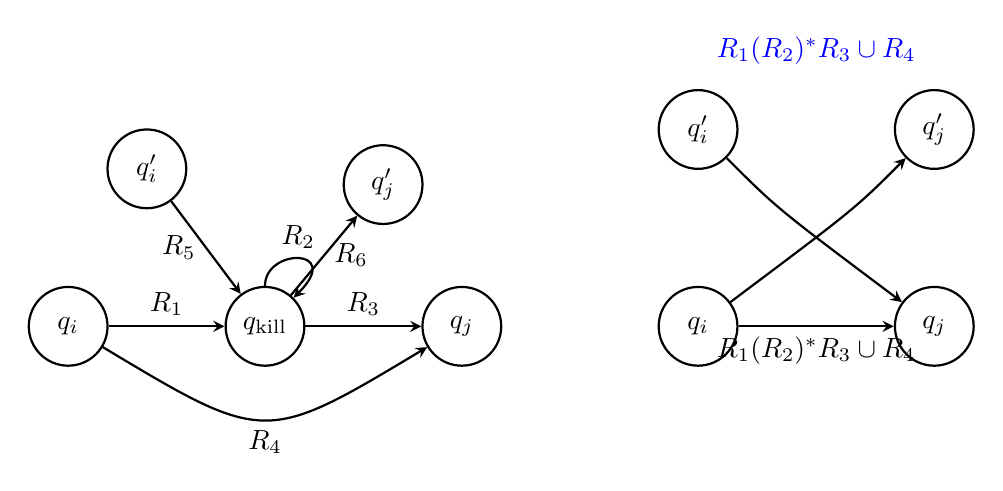
\begin{tikzpicture}[
    thick,
    >=stealth
]

% Left diagram
% States
\node[circle,draw,minimum size=1cm] (qi1) at (0,0) {$q_i$};
\node[circle,draw,minimum size=1cm] (qkill) at (2.5,0) {$q_{\text{kill}}$};
\node[circle,draw,minimum size=1cm] (qj1) at (5,0) {$q_j$};

% Top states
\node[circle,draw,minimum size=1cm] (qi_prime1) at (1,2) {$q'_i$};
\node[circle,draw,minimum size=1cm] (qj_prime1) at (4,1.8) {$q'_j$};

% Self-loop on qkill
\draw[->] (qkill) .. controls (2.5,1) and (3.5,1) .. node[above] {$R_2$} (qkill);

% Main transitions
\draw[->] (qi1) -- node[above] {$R_1$} (qkill);
\draw[->] (qkill) -- node[above] {$R_3$} (qj1);
\draw[->] (qi1) .. controls (2.5,-1.5) .. node[below] {$R_4$} (qj1);

% Top transitions
\draw[->] (qi_prime1) -- node[left] {$R_5$} (qkill);
\draw[->] (qkill) -- node[right] {$R_6$} (qj_prime1);

% Right diagram (simplified)
% States
\node[circle,draw,minimum size=1cm] (qi2) at (8,0) {$q_i$};
\node[circle,draw,minimum size=1cm] (qj2) at (11,0) {$q_j$};

% Top states
\node[circle,draw,minimum size=1cm] (qi_prime2) at (8,2.5) {$q'_i$};
\node[circle,draw,minimum size=1cm] (qj_prime2) at (11,2.5) {$q'_j$};

% Main transition with label
\draw[->] (qi2) -- node[below] {$R_1(R_2)^*R_3 \cup R_4$} (qj2);

% Curved arrows
\draw[->] (qi_prime2) .. controls (9,1.5) .. (qj2);
\draw[->] (qi2) .. controls (10,1.5) .. (qj_prime2);

% Title above right diagram
\node[text=blue] at (9.5,3.5) {$R_1(R_2)^*R_3 \cup R_4$};

\end{tikzpicture}

\newpage
Regular Expressions In Practice:
\begin{itemize}
  \item Used widely for pattern-matching, searching.
  \begin{itemize}
    \item Specify the format of a string such as a phone number, address, credit card number, license plate \dots
    \item Search a document to see if it contains some credit card number.
  \end{itemize}
  \item What algorithm is used: 
  \\ regex $\rightarrow$ NFA $\rightarrow$ DFA
\end{itemize}

\newpage
\subsection{Non-Regular Languages (Pumping Lemma)}
Not all languages are regular. Consider:
$L = \{ 0^n 1^n \: : \: n \geq 0 \} \:\:(\text{e.g. 0011} \in L \text{ but 001 } \notin L)$
\begin{theorem} \label{theo:pumping}
  Intuition: A DFA for L would need to remember how many 0's it has seen. Not enough memory
\end{theorem}
Our Plan:
\begin{itemize}
  \item Direct proof that $L = \{ 0^n 1^n \: : \: n \geq 0 \}$ is not regular
  \item Generalize the above ideas to "pumping lemma"
  \item Use "Pumping Lemma" to prove several other languages are not regular.
\end{itemize}
\begin{proof} \ref{theo:pumping}
  Assume by contradiction there is a DFA $M$ that recognized $L$. Let number of states in M = $p$.
  \\ Let $r_k \in Q$ be the state M reaches after reading $0^k$.
  \\ Then for some $0 \leq i \leq j \leq q$ we have $r_i = r_j$. 
  \\ M must accept $0^i 1^i \in L$.
  \\ $\Rightarrow$ M accepts $0^j 1^i \notin L$.
\end{proof}

\begin{lemma}
  Pumping Lemma:
  \\ If L is a regular language, then:
  \\ $\exists p \in \mathbb{Z}, p \geq 0$ (pumping length)
  \\ $\forall \text{strings }w \in L$ of length $|w| \geq P$
  \\ $\exists$ strings x,y,z $: w = xyz, |y| > 0, \: |xy| \leq p$
  \\ $\forall i \in \mathbb{N}, xy^iz \in L$.
\end{lemma}

To prove L is not regular, use contrapositive:
\begin{definition} \label{def:contrapositive}
  Contrapositive: $A \Rightarrow B = \neg B \Rightarrow \neg A$
\end{definition}
Recall De Morgan's law:
\begin{definition} \label{def:demorgan}
  $\neg \forall x \phi(x)$ is the same as
\end{definition}

\begin{figure}[htp]
  \centering
  \includegraphics[width=12cm]{"pumpinglemma.png"}
\end{figure}

Recall that the pumping lemma requires you to give a strategy for winning the following game:
\begin{itemize}
  \item The adversary chooses some integer $p$.
  \item You choose a string $w \in L$ such that $|w| \geq p$.
  \item The adversary chooses strings $x,y,z$ such that $w = xyz$ and $|xy| \leq p, |y| \geq 1$.
  \item You choose an integer $i$ and you win if $xy^iz$ is not in $L$.
\end{itemize}
Therefore, for each language you ONLY need to answer the following questions (be concise):
\begin{enumerate}
  \item What's your strategy for choosing the string $w$ in the above game?
  \item What's your strategy for choosing  the integer $i$ in the above game?
  \item How do you know that $xy^iz$ is not in $L$? 
\end{enumerate}
To show L is not regular, show:
\begin{enumerate}
  \item $\forall p \in \mathbb{N}$
  \item $\exists \text{ strings } w \in L$ of length $|w| \geq P$
  \item $\forall \text{ strings } x,y,z \: : \: w = xyz, |y| > 0, |xy| \leq p$
  \item $\exists i \in \mathbb{N}, x y^i z \notin L$
\end{enumerate}
\newpage
\section{October 3}
\subsection{Turing Machines}
"If you want to learn anything about automata you can just ask chatGPT"
\\
A Turing machine is a General Model of Computation
\begin{itemize}
    \item \textbf{Algorithms have been around since dawn of time.}
          \begin{itemize} 
            \item Long addition, multiplication, division.
            \item Compass and straightedge constructions 
            \item Euclid's greatest common divisor algorithm  
            \item Quadratic formula: finding roots of polynomials
          \end{itemize}
    \item Traditionally, algorithms were understood as a human construct. No precise mathematical definition.  
\end{itemize}
Already saw a limited notion of algorithms (DFA). Using the pumping lemma, we proved that there are some problems that are not computable in this model.
\subsubsection{David Hilbert's Descision Problem}
In 1928, David Hilbert asked for an "algorithm" that takes as input a mathemattical statement and decides whether the statement is \underline{true} or \underline{false}.
\\
During the years 1931-1936, a series of works showed there is no algorithm for the decision problem.
\\
Each of these works included a different definition of a \underline{"general algorithm"}.
\begin{itemize}
  \item Kurt Godel relied on recursive functions.
  \item Alonzo Church developed $\lambda$-calculus.
  \item Alan Turing developed the Turing Machine.
\end{itemize}
All of these definitions turn out to be equivalent.
\\
Turing Machines are perhaps the most intuitive. They provided inspiration for a general computer, the \underline{Von Neumann Architecture}
\newpage
\subsubsection*{Turing Machines cont.}
Our Plan
\begin{itemize}
  \item Define Turing Machines (TM). See how they work.
  \item Convince ourselves that TMs are powerful enough to implement any "reasonable algorithm".
    
\end{itemize}
A TM is like a DFA with infinite memory tape. Information can be saved and accessed using the tape instead of the DFA's state space.
\begin{itemize}
  \item Initially, tape contains the input, followed by "blanks". The tape head is at the left-most position.
  \item In each step, the machine can overwrite the symbol under the tape-head and move the tape left or right.
    \begin{itemize}
      \item The tape head cannot move left of the start.
      \item TMs can use additional symbols to write to tape.
    \end{itemize}
  \item At any point in time, the machine can halt the computation and \underline{accept} or \underline{reject}. (If there is no decision edge at the state the head is on, also reject)
  \item This is implemented via states and transitions like a DFA
\end{itemize}
\begin{definition} \label{TuringMachine}
  A \underline{Turing Machine} consists of a tuple: 
  \\$M = (Q, \Sigma, \Gamma, \delta, q_{start}, q_{accept}, q_{reject}$) Where
  \begin{itemize}
    \item Q is a finite set called the \underline{states}. 
    \item $\Sigma$ is an \underline{input alphabet}.
    \item $\Gamma$ is the \underline{tape alphabet} such that $\Sigma \subseteq \Gamma$ and $\Gamma$ contains a special blank symbol '-' that is not in $\Sigma$.
    \item $q_{start} \in Q$ is the \underline{start state}.
    \item $q_{accept} \in Q$ is the \underline{accept state}, $q_{reject}$ is the reject state.
    \item $\delta : Q' \times \Gamma \rightarrow Q \times \Gamma \times \{L, R\}$ is the \underline{transition function}.
    \\ \indent \indent Where $Q' = Q \setminus \{q_{accept}, q_{reject}\}$
  \end{itemize}
\end{definition}


\newpage
\section{October 7}
\subsection{Building a Turing Machine}
\begin{definition}
  \textbf{Configuration} encodes all information about a particular step in the computation of a turing machine.
  \\
  All information:
  \begin{itemize}
    \item Current state
    \item Content on the tape
    \item Tape-head position
  \end{itemize}
  Let $M = (Q, \Sigma, \Gamma, \delta, q_{start}, q_{accept}, q_{reject}$ be a Turing Machine.
  \begin{itemize}
    \item A \textbf{configuration} of M is a tuple $C=(u,q,v)$ such that $u,v \in \Gamma^{*}$ and $q \in Q$. Can write $C=uqv$ without commas.
    \item A configuration $C$ \textbf{yields} $C'$ if M goes from C to C' in 1 step.
    \begin{itemize}
      \item $C = (u, q, bw)$ yields $C' = (ub', q', w)$ if $\delta(q,b) = (q', b', R)$
      \item $C = (ua, q, bw)$ yields $C' =  (u,q',ab'w)$ if $\delta(q,b) = (q', b', L))$
      \item $C = (q,bw)$ yields $C' = (q',b'w)$ if $(q,b) = (q', b', L)$ (don't fall off)
    \end{itemize}
    \item A start configuration of M on input W is $q_{start}W$
    \item An accepting (resp.  rejecting) configuration is one where the state is $q_{accept}$ (resp.  $q_{reject}$). 
  \end{itemize} 
  M accepts (resp. rejects) w if there is a sequence of configurations $C_1, C_2, ... , C_n$ such that:
  \begin{itemize}
    \item $C_1$ is the start configuration of M on input w.
    \item $C_i$ yields $C_{i+1}$ for $i = 1,...,n-1$.
    \item $C_n$ is an accepting (resp. rejecting) configuration.
  \end{itemize}
\end{definition}
This is a way to save your current state for later.
\\
If $C = (ua, q, bv), \: \delta(a, b) = (q', c, L)$, then $C' = (u, q', acv)$
\\
If $\delta(a, b) = (q', C, R)$ then $C' = (uac, q', v)$

\newpage
\section{October 10}
\subsection{Language of a TM}
\begin{itemize}
  \item A TM M on input w can either accept, reject, or loop
  \item For a TM M, we define $L(M) = \{w | M \text{ accepts } w \}$
  \item If TM M and a language L satisfies "for any $x \in L$, M accepts x", we cannot say "M recognizes L". We must prove that $L(M) = \{w | M \text{ accepts } w \}$ 
  \item \quad Do this using $\subseteq$ (M accepts any string in L) and $\supseteq$ (If a string is accepted by M, the string is in L).
  \item We say the M \textbf{decides} L if 
  \begin{itemize}
    \item M accepts $w \in L$ and M rejects $w \notin L$.
    \item equivalently: M recognizes L and M always halts.
  \end{itemize}
  \item A language L is \textbf{recognizable} (resp. \textbf{decidable}) if there is some TM that recognizes (resp. decides) L.
  \item The set of all languages decided by turing machines is a subset of all languages recognized by turing machines.
\end{itemize}

\subsection{Specifiying a Turing Machine}
Instead of drawing a state diagram, we give a "tape-head" level description that abstracts out the states/transitions via pseudocode.
\begin{itemize}
  \item Imagine tape-head has small local memort which is "fixed" and cannott grow with input size (states of TM).
  \item Describe how the tape-head should \textbf{walk across the tape} and \textbf{what it should write}.
\end{itemize}
\begin{example}
  $L = \{a^{2n} | n \geq 0\}$ all powers of 2.
  \\
  Walk tape-head from left to right and cross out any other a.
  \begin{itemize}
    \item If tape contained a single 0, accept.
    \item Else if number of 0s was odd, reject.
    \item Else return to the left-hand end of tape, repeat. 
  \end{itemize}
\end{example}
\begin{example}
  $L = \{ w \# w: w \in (0,1)^{*} \}$
  \begin{itemize}
    \item Check input is of form $\{0, 1\}^* \# \{0, 1\}^*$ and reject otherwise.
    \item 
  \end{itemize}
\end{example}

\subsection{Beyond Boolean Functions}
We can also consider TM's that output more than just "accept/reject"
\\
Idea: define the output of a TM as the contents of its tape when it enters a halt state.
\\
A TM M computes a function $f: \: \Sigma^* \to \Sigma^*$ if on every input $w \in \Sigma^*$ the TM \textbf{halts} and its tape contains f(w).

\begin{definition}
  We say that f is \textbf{computable} if some TM M computes it.
\end{definition}
\begin{example}
  $f: \: \{0, 1\}^* \to \{0, 1\}^*$: f(binary rep of n) = binary rep of n + 1. f is the binary successor function.
  \\ 
  Show that this is computable.
  \\
  Given any input string such as '01101101111':
  \\
  Move to the end of the string and continue left until the beginning. Flip all 1's until the first 0, flip the first 0.
  \\
  To prevent crashing off the beginning of the tape if all ones: convert first character to a \# if it is a 1 and add a zero on the end if it is reached.
\end{example}
\newpage
\section{October 14 - Turing Machine Variants}
\subsection*{Multi-Tape TM}
A TM with one input tape and multiple work tapes. Transition function is defined by $\delta = Q' \times T \to Q \times T \times \{L, R\}$.   $\delta(g, w) = (g', w, L/R)$.
\begin{itemize}
  \item You can concatenate multiple tapes to one tape and separate their contents by \#. 
  \item Remember tape-head positions by storing an \underline{underlined} version of tape symbols. 
  \item Each step of multi-tape TM is simulated by scanning entire tape of single-tape TM.
  \item If you run out of space on the tapes, shift all elements to the right. (halting problem)
\end{itemize}
Tape-Head Level Description:
\\
f(a, b) = a + b. Input (binary interpretations of two integers separated by a \#)
\begin{itemize}
  \item Reverse each input and copy each one to a different tape and clear main tape. 
  \item Return all tape heads to the left. Store 1-bit carry as 0
  \item Add two bits under each tape head (using 0 if one head is empty) and carry bit:
    \begin{itemize}
      \item Write result mod 2 to the main tape.
      \item Move all tape heads 1 right.
      \item Repeat until both heads are empty.
    \end{itemize}
  \item Reverse main tape.
\end{itemize}

\subsection*{Random Access TM}
Can read/write to arbitrary locations in memory without scanning a tape. Memory modeled as infinite array R.
\begin{itemize}
  \item In addition to the standard tape that contains the input the TM has location and value tapes.
  \item There is a special write transition which sets R[location] = value using the content of the tapes.
  \item There is a read transition which sets the contents of the values tape to R[location]
\end{itemize}
Compliling to normal TM:
\\
We use a multi-tape machine (which can be converted to a single-tape)
\begin{itemize}
  \item Store contents of array R on a tape as tuples (location$_n$, value$_n$).
  \item To simulate a read, scan R until find a location that matches content of location tape. Write the value on the value tape. Put a blank if no such value is found.
  \item To simulate a write, scan R until you find location that matches content of location tape. Update value. If none found, append (location, value) to end of R.
\end{itemize}
\subsection*{Turing Completeness}
\begin{theorem}
  Church-Turing Thesis: Any algorithm (in an informal sense) can be computed by a TM.
\end{theorem}
Proof Outline:
\\
Design a compiler that converts Java program into a TM.
\begin{itemize}
  \item All programming languages are already compiled to "assembly code" for modern CPUs
  \item Assembly code instructions can be implemented on a Random-Access TM.
\end{itemize}



\end{document}
